
\chapter{Evaluation}\label{chapter:evaluation}

%\subsection{Design}

%Our design is constructed as follows. We generate different graph topologies with different densities and achieve a deviation in their %representative metrics, especially concentrating on the clustering coefficient, betweenness centrality and average shortest path. Our assumption is %that these metrics affect mostly and characterize the performance. We investigate the relationships between metrics and performance in the graphs %that contain the same number of nodes. 

\section{Benchmarking Environment}

The benchmarking environment involves a single machine that contains a quad-core Intel Xeon Processor L5420 (2.5 GHz) and 16 GBs of RAM. In order to alleviate the effect of transient on the measurements and minimize the noise in the results, a 64-bit Ubuntu 14.04.2 LTS was installed. Additionally, Oracle JDK version 1.8.0 was used as the Java environment.


\section{Benchmark Configuration}

\paragraph{Topologies}

We generate five topologies for the measurements such as the scale-free model, hierarchical network and Watts-Strogatz models with different probability $p$ values as $0.1$, $0.01$ and $0.001$. Due to these configurations of $p$, we reach a deviation between Watts-Strogatz models and random graphs.\\ The topologies are generated via our uniform model generation approach (Section \ref{sec:uniform_generation}).
Every topology is generated five times with different densities that are adjusted to five different values based on the size of $K_n$ complete graphs found in the hierarchical network. These $K_n$ complete graphs are configured to $K_3$, $K_4$, $K_5$ $K_6$ and $K_7$.

\paragraph{Queries}
The queries are parameterized with random values 20 times and executed on every graph. Each measurements is performed 4 times.

\paragraph{Model Size}

The configuration of the model sizes are shown in Table \ref{tab:graph_size} representing number of nodes and edges. The latter is given by an interval since we generate the graph with different densities.

\begin{table}[ht]
	\footnotesize
	\centering
	
	\begin{tabular}{ l c c c}
		\toprule
		Nodes & Min Edges & Max Edges \\ \hline
		%		\midrule 
		5~000 & 23~531 & 42~633\\ \hline
		10~000 & 49~140 & 89772\\ \hline	
		20~000 & 100656 & 185420\\ \hline
		40~000 & 209439 & 381435\\ \hline
		80~000 & 421110 & 800314\\ \hline
		\bottomrule
	\end{tabular}
	\caption{The number of nodes and edges in generated graphs.}
	\label{tab:graph_size}
\end{table}

\section{Samples}

In order to analyze the relationships between model metrics and the performance of query evaluations, we create different samples of the measurements and investigate them respectively. The triple of a specific tool, query and model size (number of nodes) defines a sample. A sample contains the measurement results for a particular query evaluated by a tool on a model of a certain size. As a result, the number of different samples is equal to the product of unique tools, queries and model sizes.

\subsection{Sample Size}
A sample includes the measurements executed on 5 different topologies, each of them appears 5 times in the sample with different densities that are configured between the various topologies equally. One sample contains 20 evaluations of a parameterized query. Every measurement is repeated 4 times in a sequence, however, we discard the first evaluation times and use the median of the remaining measurements.\\
The dimensions in a sample and their occurrences are illustrated in Table \ref{tab:sample_size}. Since the triple of a tool, query and model size defines a different sample, these values represent one value in a sample. As it can be observed, the sample size is equal to $500$.

\begin{table}[ht]
	\footnotesize
	\centering
	
	\begin{tabular}{ l c c c c c c || c }
		\hline
		 & Tool & Query & Model Size & Query Evaluation & Topology  & Density & $\prod$\\ [5pt] \hline
%		\midrule 
		Occurrence & 1 & 1 & 1 & 20 & 5 & 5 & 500 \\ \hline
%		\bottomrule
	\end{tabular}
	\caption{The dimensions and their occurrence in a sample.}
	\label{tab:sample_size}
\end{table}


\section{Model Analysis}

\subsection{Density}
One essential expectation was in our work to generate different graphs with the same number of nodes and edges. Figure \ref{fig:density} depicts the density of the topologies. The $x$-axis represents the sizes of the models, the $y$-axis shows the values belonging to density. Every column contains the information of one specific topology, furthermore, the different densities are separated by colours in the legend.
\begin{figure}[!ht]
	\centering
	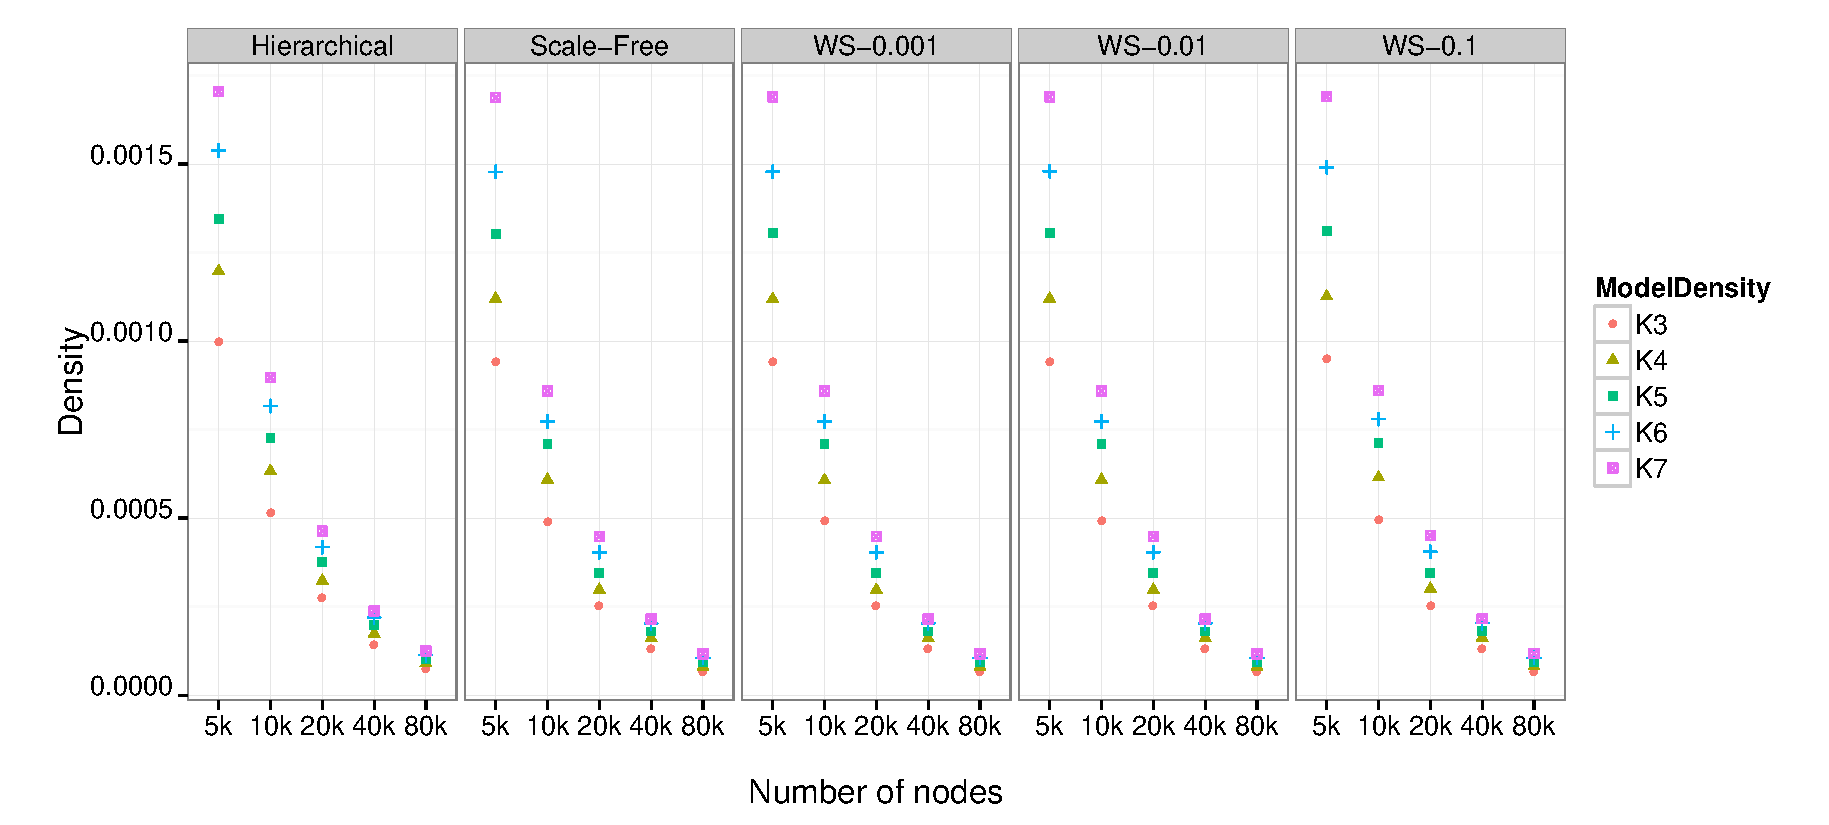
\includegraphics[width=160mm, keepaspectratio]{figures/density.pdf}
	\caption{The density of the graph topologies.}
	\label{fig:density}
\end{figure}

As it can be observed, the topologies with different networks have approximately the same density with the respect to the number of nodes, which implies the number of edges is almost equal. A small deviation is shown between the hierarchical graph and the other topologies. This is explained by the fact that the recursive generation algorithm of the hierarchical network must be terminated before its end in order to obtain an arbitrary number of nodes. Hence, we can only estimate the amount of edges in the graph with a dispersion. The standard deviation of the densities is $1.11 \cdot 10^{-5}$, and divided by the maximum number of density we obtain 0.028, which means a 2.8\% difference between the topologies with respect to their density.

\subsection{Clustering Coefficient}

Our goal is to achieve a deviation in metric values per topologies such as the clustering coefficient metric. Figure \ref{fig:clustering_metric} depicts the average clustering coefficients in the topologies. The $x$-axis represents the number of nodes in the graphs, the $y$-axis denotes the values of the metric, furthermore, every value is separated by the topology in legend.\\
The plot shows how the values spread in the $[0,1]$ interval according to our early expectation (Section \ref{sec:topology_metric}). One topology has more corresponding metric value in the same size---\eg hierarchical---due to the fact that we generated 5 instances of every topology with different densities, which implies a different clustering coefficient metric per instance as well.

\begin{figure}[!ht]
	\centering
	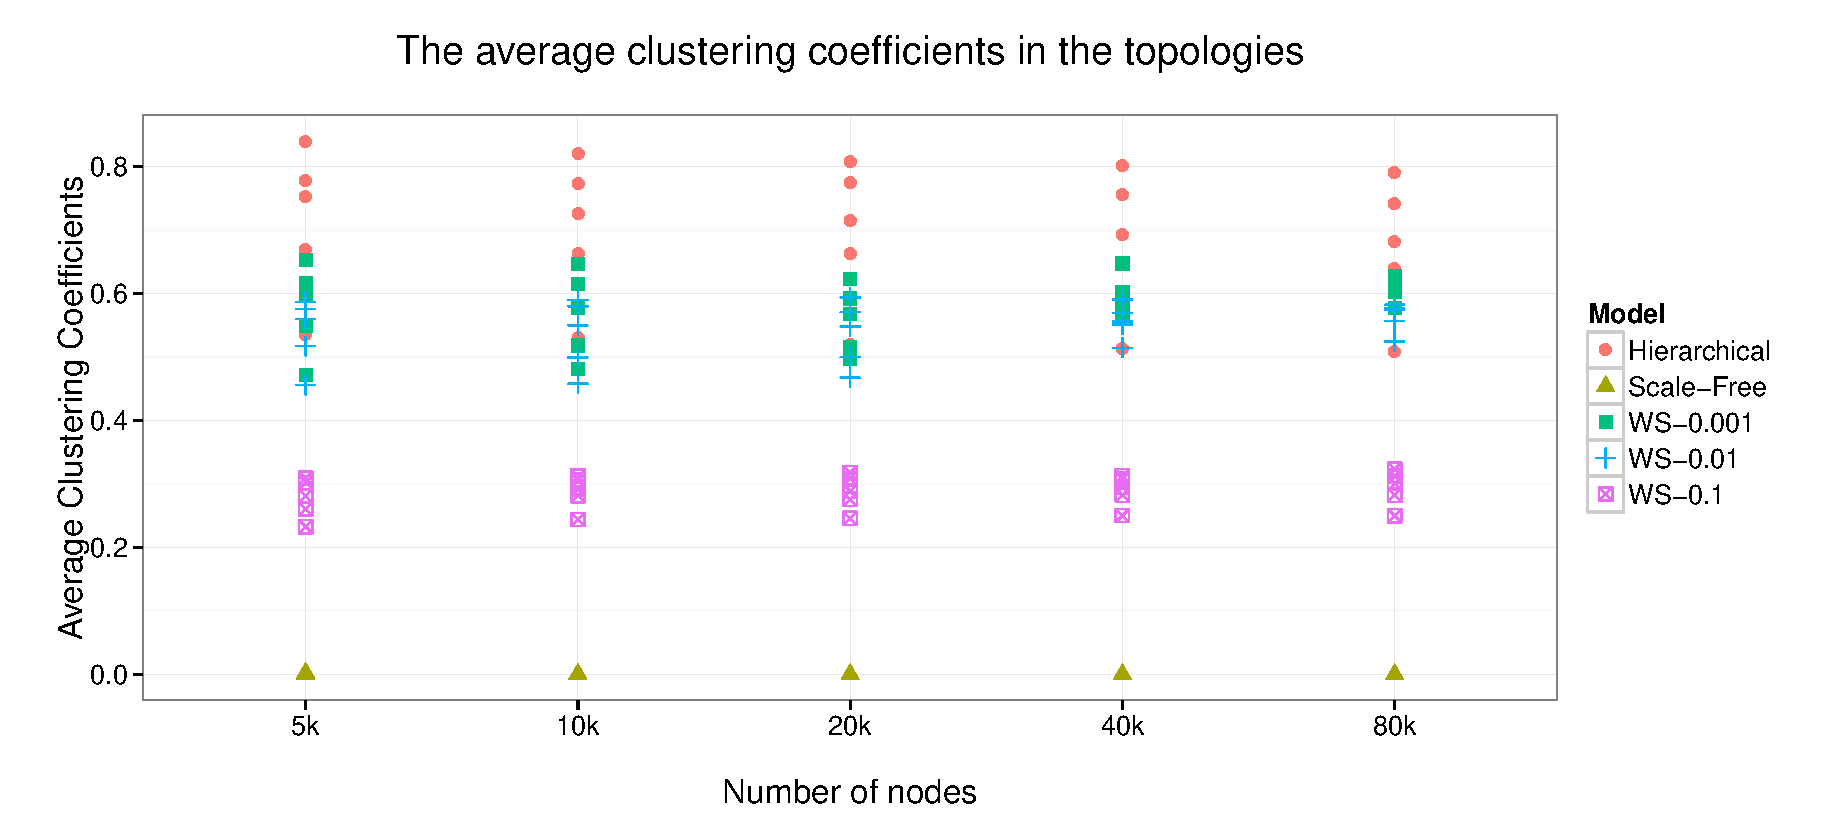
\includegraphics[width=160mm, keepaspectratio]{figures/clustering_metric.pdf}
	\caption{The average clustering coefficient in the graph topologies.}
	\label{fig:clustering_metric}
\end{figure}

\subsection{Shortest Path Length}

The average lengths of shortest paths in the topologies are demonstrated in Figure \ref{fig:betweenness_metric}. It can be observed that as we decrease the $p$ probability in the Watts-Strogatz models (from $0.1$ to $0.001$), the lengths of the shortest paths increase. This negative correlation shows the same results that we expected and can be explained by the operation of the generation algorithm belonging to the Watts-Strogatz model. As we increase the $p$ value, the algorithm rewires every edge with $p$ probability---\ie it deletes an edge and connects it to a new random node---and this entails a bigger interconnectivity in the graph showing a small-world property. On the contrary, a low $p$ value (\eg 0.001) modifies a subtle set of the edges, therefore, the graph still shows similar characteristics than a lattice graph with high average shortest path length.

\begin{figure}[!ht]
	\centering
	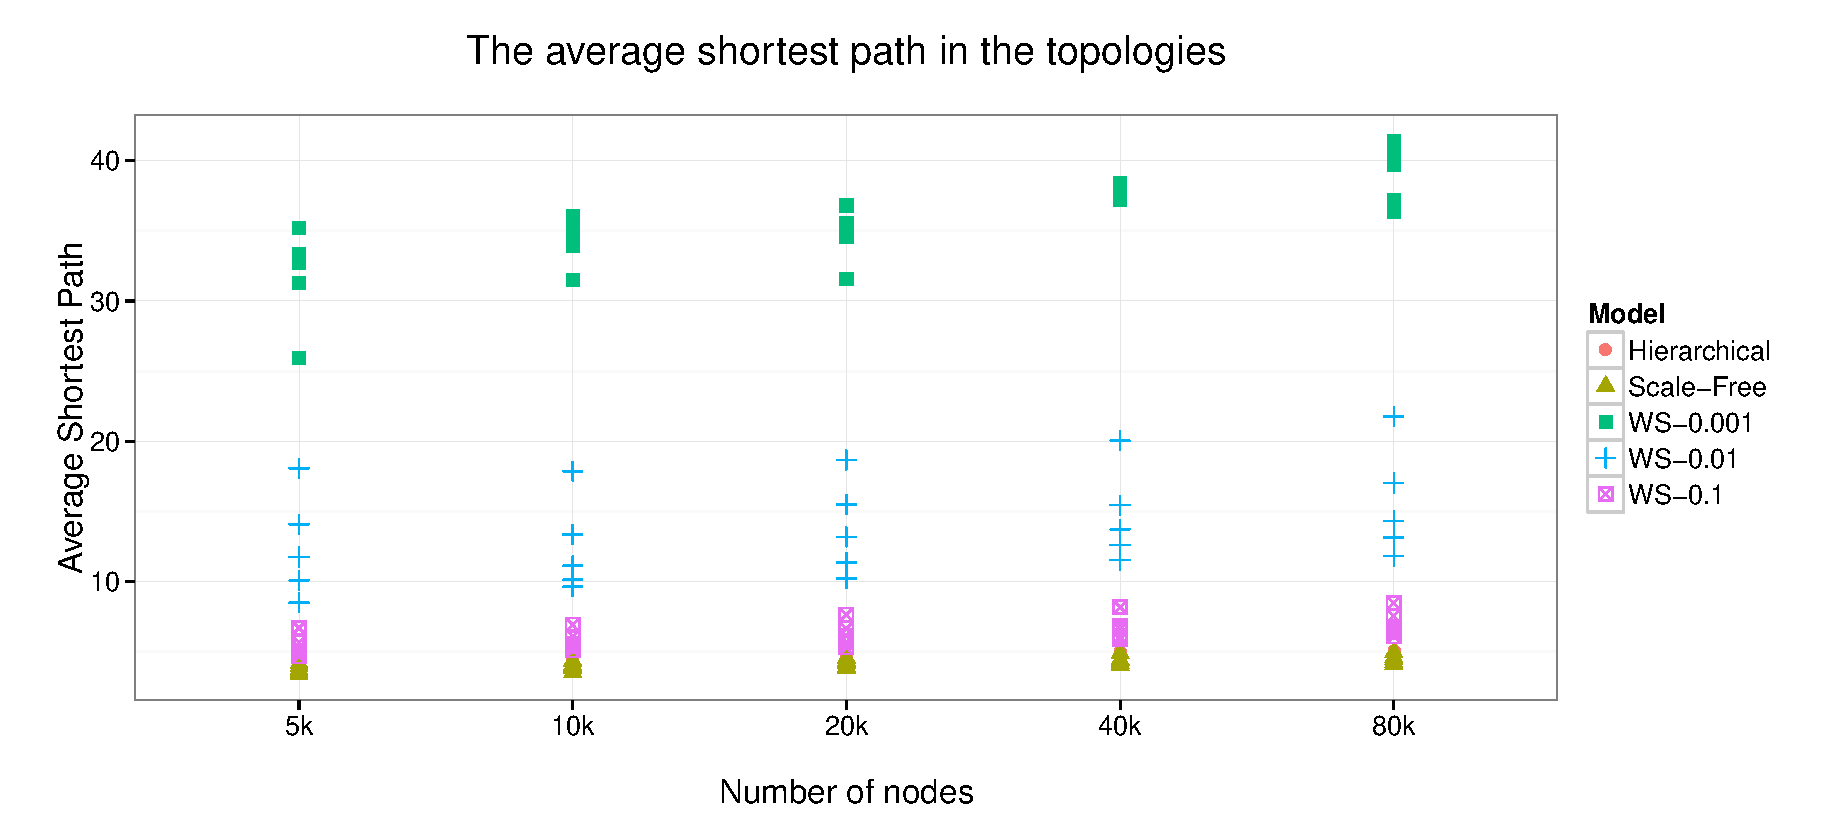
\includegraphics[width=160mm, keepaspectratio]{figures/avg_sp_metric.pdf}
	\caption{The average shortest path in the graph topologies.}
	\label{fig:avg_shortest_path}
\end{figure}

\subsection{Betweenness Centrality}

Figure \ref{fig:betweenness_metric} illustrates the betweenness centrality metric per topologies. Regarding this metric, we assumed a more significant deviation among the topologies, as we expected that the \emph{hubs}---the nodes with higher degrees---in scale-free models appear more times in the shortest paths implying a higher betweenness centrality. Instead, the WS-0.001 model shows higher values in this metric than the scale-free model except in the case of the largest graph.\\
A gap is observed between the hierarchical network and the other topologies due to the fact the center node in the hierarchical graph dominates the calculation of the betweenness centrality metric.

\begin{figure}[!ht]
	\centering
	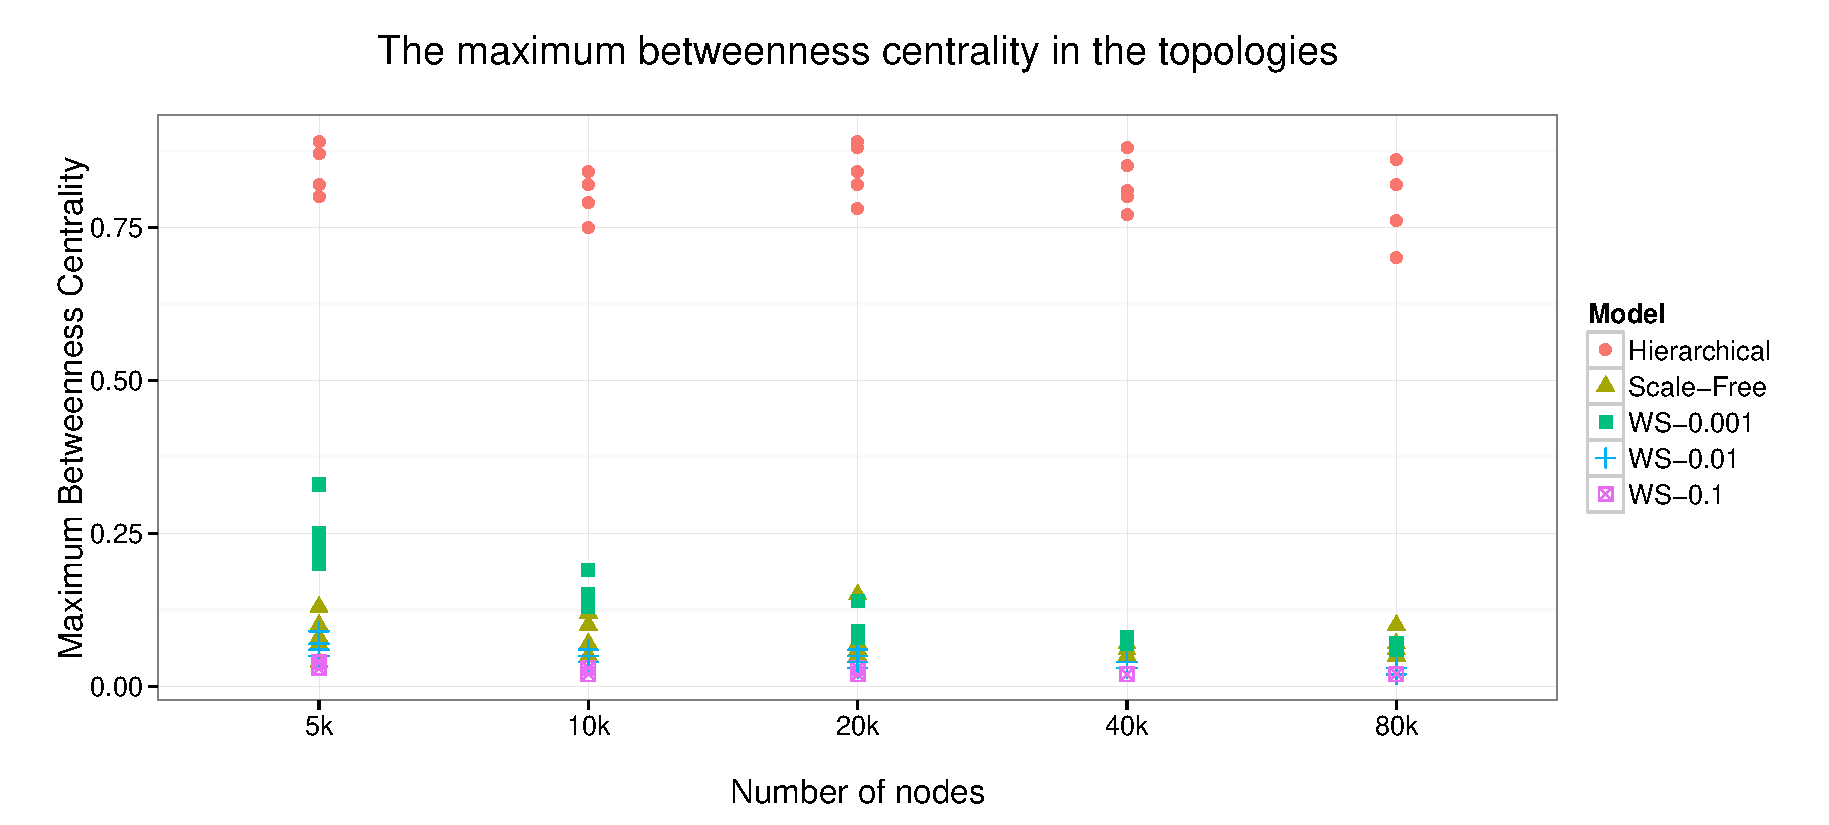
\includegraphics[width=160mm, keepaspectratio]{figures/betweenness_metric.pdf}
	\caption{The maximum betweenness centrality in the graph topologies.}
	\label{fig:betweenness_metric}
\end{figure}

\section{Performance Analysis}

\subsection{Hypothesis}

Our hypotheses about the results of query evaluations are the following.

\paragraph{Reachability Query}
Regarding the first query---Reachability---we assume that the larger clustering coefficients and higher degrees may cause a performance loss of the tools. If the graph has a higher clustering coefficient then there is a possibility that the execution of the query revisits a certain node more times via its neighbors. This implies that the evaluation contains more---unnecessary---navigations.\\
A node with higher degree also can affect the performance, since if the graph traversal visits this certain node with higher degree than there is a possibility that it also investigates its neighbors. Nodes with high degree typically appear in the scale-free models---the hubs---and the hierarchical networks---the center nodes.

The assumption comes naturally that the average shortest path length also can dominate the execution time. Among the different Watts-Strogatz models, the ones with lower $p$ values include a higher average shortest path metric, suggesting a growing in the evaluation time. However, considering the other topologies as well, it cannot be determined forward which specific characteristic dominates better.

\paragraph{Navigations Query}

The Navigations query searches nodes in three-hop distances starting from a random vertex. We believe that the nodes with higher degrees impact the performance mostly, namely, the center nodes in the hierarchical graph and the hubs in the scale-free models. We fundamental question is that whether our defined metrics are suitable to characterize the performance appropriately or not.

\subsection{Highlights of the Analysis}

For the performance analysis we created and measured 50 different samples, each of them contains 500 observations---\ie measurement results. In the following sections we do not intend to show the results in details of every sample, hence, we only concentrate on the samples that contain interesting or unexpected results.

\subsubsection{Blazegraph is highly sensitive to the average shortest path of the graph}

The measurement results of Blazegraph is illustrated in Figure \ref{fig:blazeq1}. The box plot~\cite{boxplot} shows the results in following dimensions. On the $x$-axis denotes the graph topologies and the $y$-axis represents the evaluation time in milliseconds on a logarithmic scale. Every column includes different results belonging to a specific model size.

\begin{figure}[!ht]
	\centering
	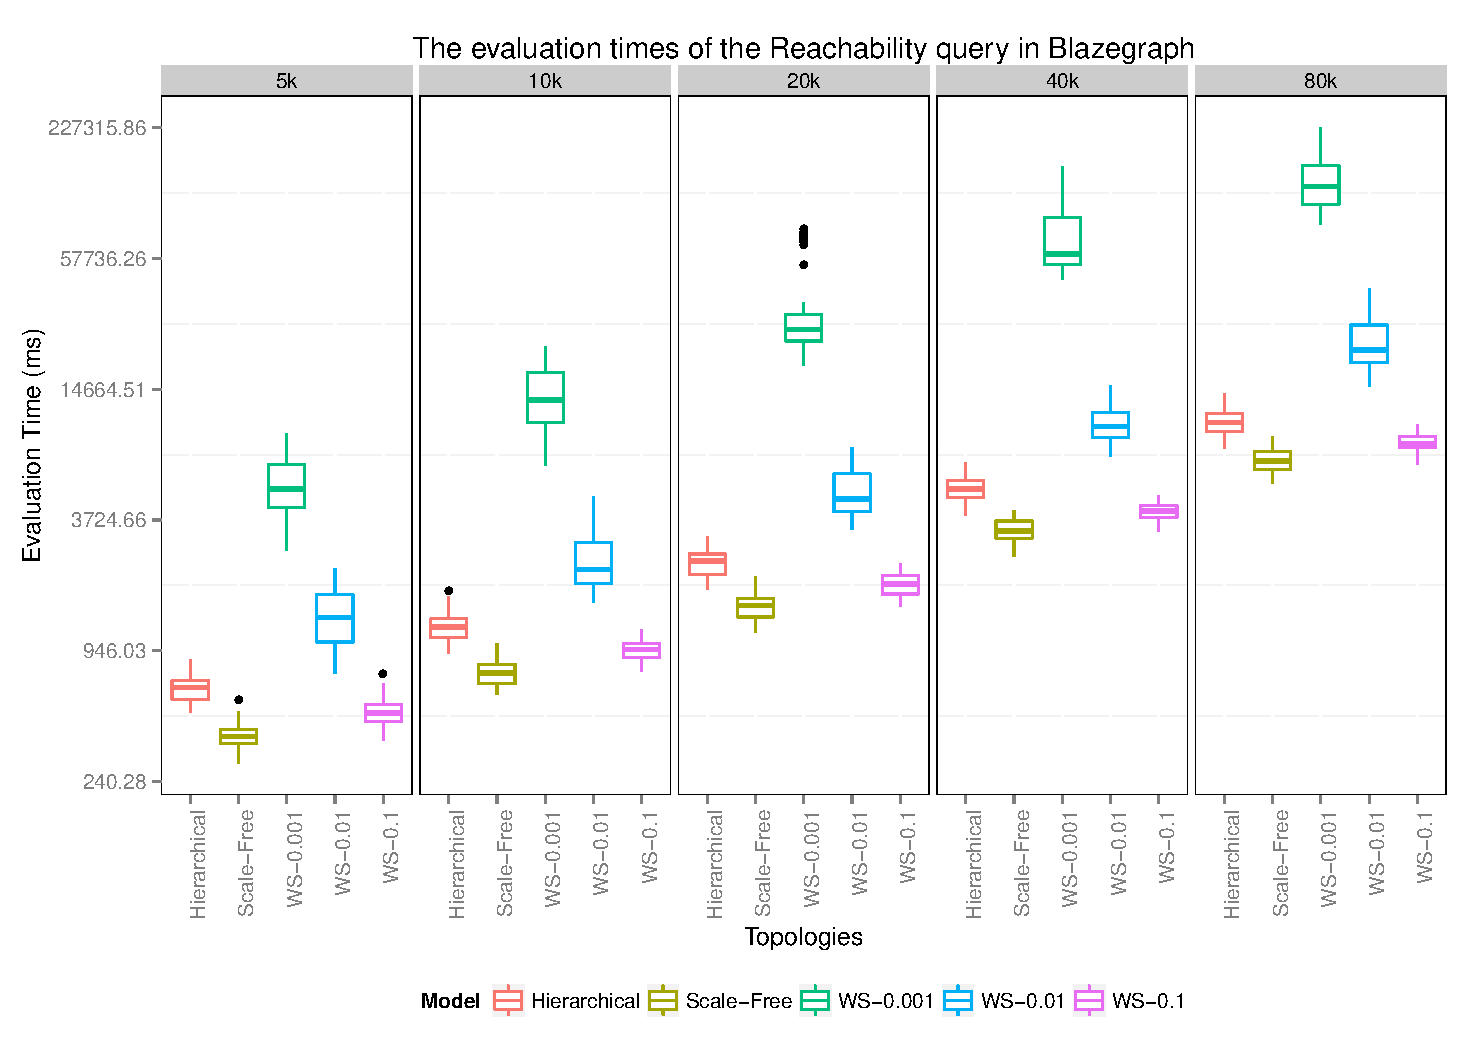
\includegraphics[width=160mm, keepaspectratio]{figures/blaze_q1.pdf}
	\caption{The measurement results of the Reachability query in Blazegraph.}
	\label{fig:blazeq1}
\end{figure}

The most important observation is the deviation in evaluation time among the topologies. Besides the execution times increases with respect to the number of nodes, the performance also varies among the networks being in the same size. A significant difference is shown between the Watts-Strogatz models (WS-$0.001$, WS-$0.01$) and the other networks.

The created regression models are listed in Table \ref{tab:regressions_blaze_a1}. Every measurement result and metric were normalized for the calculations, and the table includes the best fitted regression models on the measurements. In every case, the average shortest path metric seemed to be the best predictor. Regarding different model sizes, the value of adjusted R$^2$---\ie coefficient of determination---varies between 0.68 and 0.9 that show well-fitted regression models. 

\begin{table}[ht]
	\footnotesize
	\centering
	\begin{tabular}{ c c c c c}
		\toprule
		Model Size & Metric & Adjusted R$^2$& Regression Coefficient & P-value\\ \hline
		%		\midrule 
		5~000 & Avg Shortest Path & $0.9$ & 0.949 & $2.2 \cdot 10^{-16}$ \\ 
		10~000 & Avg Shortest Path & 0.8586 & 0.9268 & $2 \cdot 10^{-16}$ \\ 
		20~000 & Avg Shortest Path & 0.6807 & 0.8254 & $2.377 \cdot 10^{-16}$\\ 
		40~000 & Avg Shortest Path & 0.7647 & 0.8745 & $3.3\cdot 10^{-16}$ \\  
		80~000 & Avg Shortest Path & 0.7642 & 0.8745 & $3.3\cdot 10^{-16}$ \\  
		\bottomrule
	\end{tabular}
	\caption{The best fitted regression models of Blazegraph.}
	\label{tab:regressions_blaze_a1}
\end{table}

\subsubsection{Sesame is mostly unaffected by the topology of the model}

The evaluation results of Sesame are illustrated in Figure \ref{fig:sesame_q1}. As it can be observed, the optimization in Sesame is not sensitive to the different topologies, as the various characteristics of the networks still cause nearly the same evaluation time. A higher difference only occurs between the different model sizes. Interestingly, a small difference is also observable between the Watts-Strogatz models, as the $p$ values increases---implying the decrease of the average shortest path metric---the evaluation times still grow.\\
Due to the approximately equal results, we cannot create an appropriate well-fitted regression model for Sesame.

\begin{figure}[!ht]
	\centering
	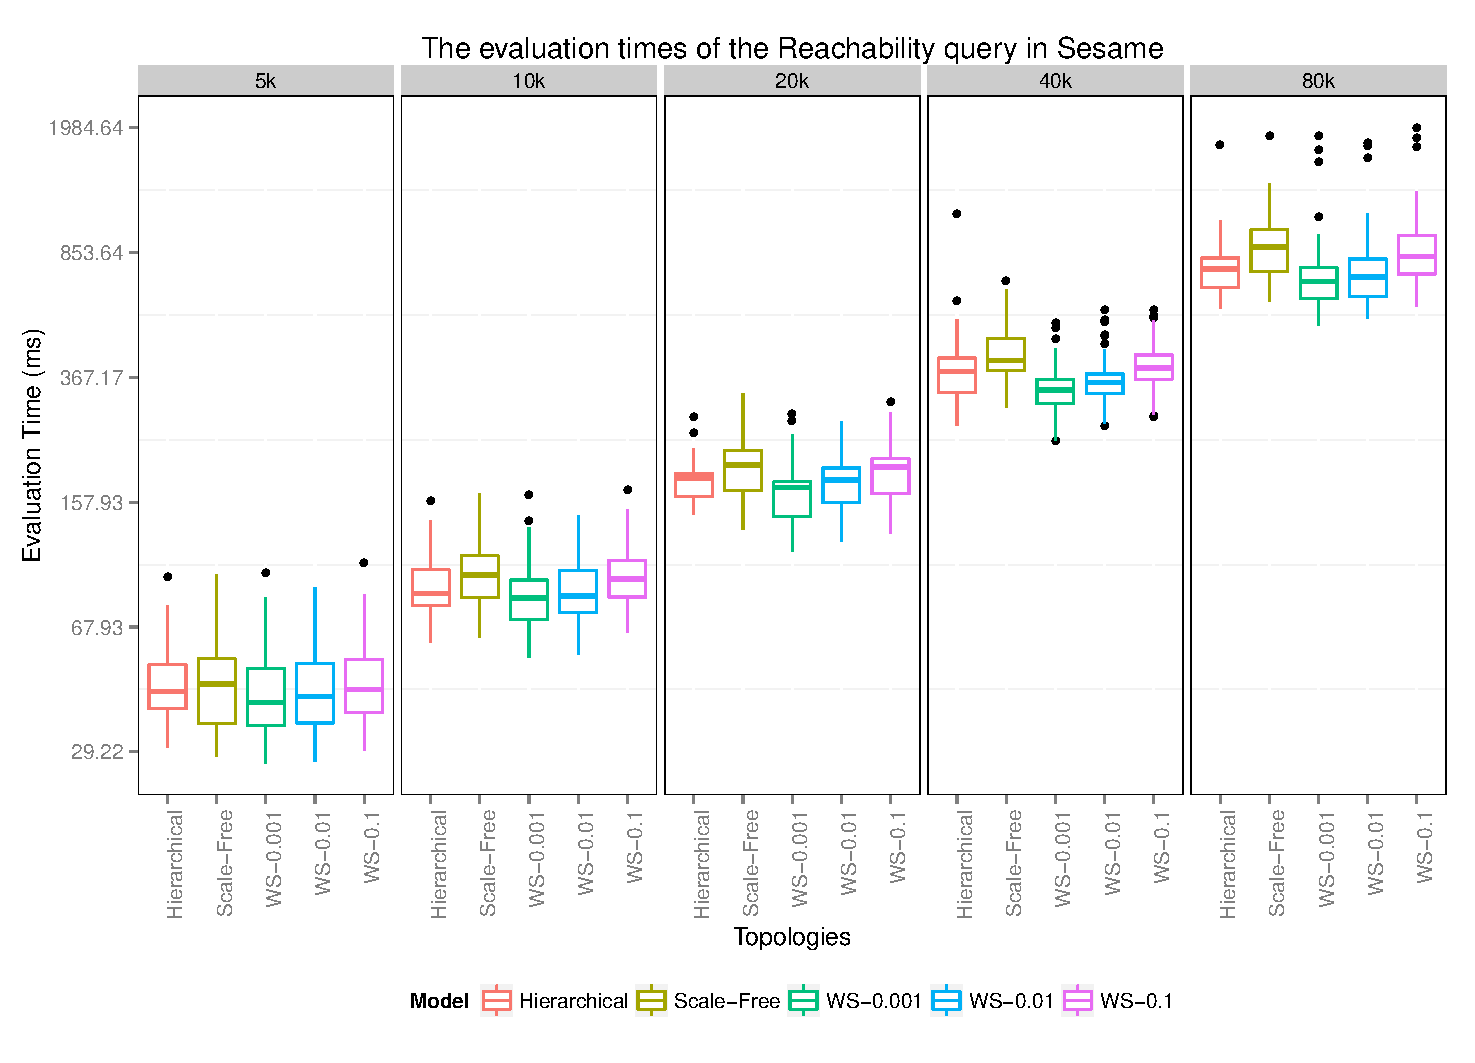
\includegraphics[width=160mm, keepaspectratio]{figures/sesame_q1.pdf}
	\caption{The measurement results of the Reachability query in Sesame.}
	\label{fig:sesame_q1}
\end{figure}

\subsubsection{The clustering coefficient does not influence the performance for the Reachability test}

Interesting to show that our assumption about the clustering coefficient metric is proved to be false. The adjusted R$^2$ values of the regression models containing the clustering coefficient are considerably small. In the case of Sesame, the adjusted R$^2$ is approximately 0.06 per different model sizes, and regarding Blazegraph, this value is equal to 0.13. Both of them indicate that the clustering coefficient has a minimal impact to the performance, in the light of these workloads.

\subsubsection{Negligible relationship between the hubs and the performance of the Reachability test}

The results of the Reachability query shows that the nodes which have significantly larger degrees do not affect the performance of the evaluations. At first sight, we would assume that the occurrence of hubs implies that the execution of the query must visits a significantly larger amount of nodes. Since, if the evaluation reaches a hub during the graph traversal than it possibly must visit its neighbors as well, causing a performance loss. However, in the case of Blazegraph, the Watts-Strogatz models with higher average shortest path lengths seem to be dominating, despite the fact that the same Reachability test in a hierarchical or scale-free network may visit more vertices than in the case of the WS models.

\subsubsection{Navigations on graphs are dominated by hubs}

The measurement results of the Navigation query is illustrated in Figure \ref{fig:fourstore_q2}. As we assumed, the hubs---\ie the significantly higher degree nodes---affect the performance of this query evaluation. A more interesting question is that whether our metrics can characterize this relationship appropriately or not. 

\begin{figure}[!ht]
	\centering
	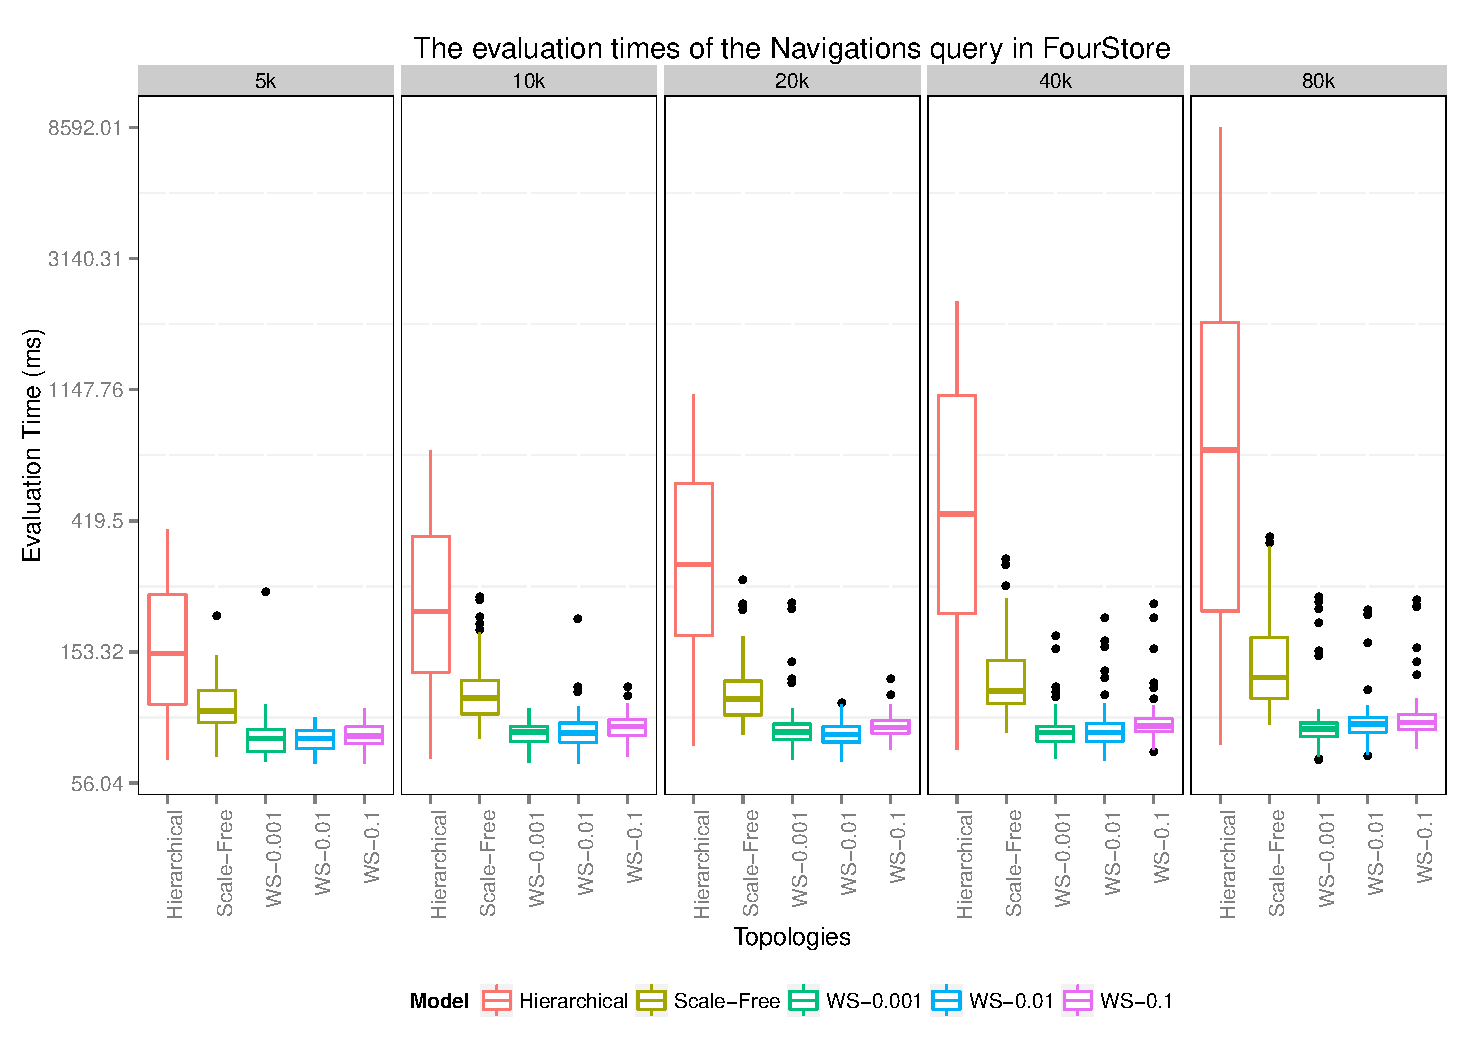
\includegraphics[width=160mm, keepaspectratio]{figures/4store_q2.pdf}
	\caption{The measurement results of the Navigations query in FourStore.}
	\label{fig:fourstore_q2}
\end{figure}

Our created regression models are shown in Table \ref{tab:regressions_4store_q2}. These are the ones that provided the best fit to the data including the betweenness centrality and maximum degree metric. The main conclusion is that our metrics partly can characterize the relationship, since the adjusted R$^2$ values vary between the 0.4396 and 0.5228 interval.
\begin{table}[ht]
	\footnotesize
	\centering
	\begin{tabular}{ c c c c c}
		\toprule
		Model Size & Metrics & Adjusted R$^2$ &  P-value\\ \hline
		%		\midrule 
		5~000 & Betweenness + Maximum Degree & 0.5228 & $2.2 \cdot 10^{-16}$ \\ 
		10~000 & Betweenness + Maximum Degree & 0.5204 & $2.2 \cdot 10^{-16}$ \\ 
		20~000 & Betweenness + Maximum Degree & 0.5125 & $2.2 \cdot 10^{-16}$\\ 
		40~000 & Betweenness + Maximum Degree & 0.4815 & $2.2\cdot 10^{-16}$ \\  
		80~000 & Betweenness + Maximum Degree & 0.4396 & $2.2\cdot 10^{-16}$ \\  
		\bottomrule
	\end{tabular}
	\caption{The best fitted regression models of Fourstore..}
	\label{tab:regressions_4store_q2}
\end{table}

As far as the other tools are concerned, such as Sesame and Blazegraph, the same metrics can be used to obtain the best fitted regression, and the adjusted R$^2$ values vary between the 0.4018 and 0.5173 interval. These results also show that only these two metrics were not adequate to characterize the performance properly regarding these workloads and samples.

\section{Conclusions}

\paragraph{Model Generation}
We showed that our model generation approach was able to construct different topologies with the same density with respect to the same number of nodes. As it was illustrated, the clustering coefficient and average shortest path length metrics were deviated appropriately among the topologies. Unfortunately, the betweenness centrality metric seemed to be dominated by the hierarchical network, and it also showed a significantly lower value in the scale-free models, than we originally expected. 

\paragraph{Performance}
The measurement results illustrated that the different internal structure of the graphs are able to cause a deviation in evaluation time, regarding the Reachability and Navigations query as well. In the first query, Blazegraph seems to be sensitive to the average shortest path length metric, on the contrary, the performance of Sesame is not affected by the topologies regarding these workloads.

\paragraph{Hierarchical Graph}

The analysis of the topologies show that the hierarchical graph has significantly different descriptive metrics than the other topologies, furthermore, our measurement results of the Navigation query also imply that the hierarchical network is overly dominating to the performance by comparing with the other networks. Our generation technique also showed that---by relying on the hierarchical graph---we cannot achieve an arbitrary density in the graph which is possible with the generation algorithms of the other topologies. We had to adapt the other networks to the limitations of the hierarchical graph. As a conclusion, the hierarchical graph is not capable to be used in our framework in the future due to its limitations.

